\documentclass[10pt]{beamer}

\usetheme{Madrid}
\usecolortheme{default}

\definecolor{primary}{RGB}{30, 58, 138}
\definecolor{secondary}{RGB}{217, 119, 6}
\definecolor{accent}{RGB}{16, 185, 129}
\definecolor{bglight}{RGB}{248, 250, 252}

\setbeamercolor{palette primary}{bg=primary, fg=white}
\setbeamercolor{palette secondary}{bg=secondary, fg=white}
\setbeamercolor{palette tertiary}{bg=primary, fg=white}
\setbeamercolor{titlelike}{parent=palette primary}
\setbeamercolor{structure}{fg=primary}
\setbeamercolor{block title}{bg=primary, fg=white}
\setbeamercolor{block body}{bg=bglight, fg=black}

\setbeamertemplate{navigation symbols}{}
\setbeamertemplate{footline}[frame number]

\usepackage{graphicx}
\usepackage{amsmath, amssymb}
\usepackage{booktabs}
\usepackage{tikz}
\usetikzlibrary{shapes.geometric, arrows, positioning}

% Title
\title[Adaptive Stopping for GANs]{Dynamic Volume Optimisation and Adaptive Stopping Criteria for GAN-Based Synthetic Data Generation}
\subtitle{Research Proposal Presentation}

\author{Group Members \\
    1. [REDACTED] -- [REDACTED] \\
    2. [REDACTED] -- [REDACTED] \\
    3. [REDACTED] -- [REDACTED] \\
}
\date{27th September 2026}

\begin{document}

\begin{frame}
    \titlepage
\end{frame}

% =========================================
% 1. INTRODUCTION
% =========================================
\begin{frame}{Background and Context}
    \begin{itemize}
        \item \textbf{Generative Adversarial Networks (GANs):} Widely used for synthetic data augmentation to solve class imbalance and data scarcity in biomedical imaging.
        \item \textbf{The Common Limitation:} Standard pipelines rely on \textit{fixed, arbitrary generation thresholds}.
        \item \textbf{The Core Problem:} Generating more synthetic data does not always mean better performance.
        \begin{itemize}
            \item Over-generation leads to \textbf{Coverage Saturation} and \textbf{Distribution Drift}.
            \item Distorts true data distributions, lowers model accuracy, and wastes compute hours.
            \item \textit{Example Observation:} Recent literature (Zhu et al.) showed soft sensor performance degrading rapidly after generating $>420$ samples.
        \end{itemize}
        \begin{figure}[htbp]
            \centering
            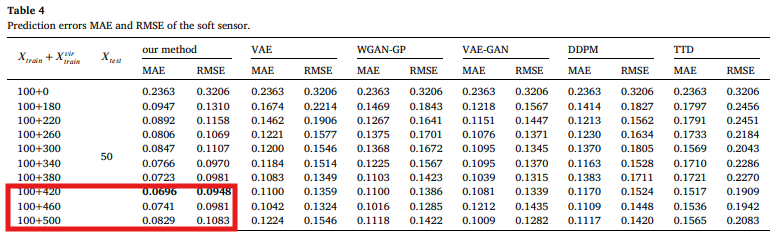
\includegraphics[width=0.7\textwidth]{distortAfter420.png}
        \end{figure}
    \end{itemize}
\end{frame}

\begin{frame}{Problem Statement}
    \begin{block}{The Core Issue}
        Arbitrary fixed thresholds cause \textbf{coverage saturation} (diminishing returns) or \textbf{distribution drift} (data distortion), degrading downstream classifier performance and wasting compute resources.
    \end{block}

    \vspace{0.3cm}

    \begin{block}{Proposed Solution}
        An \textbf{``Adaptive Comparing and Stopping''} framework integrated directly into the GAN loop to dynamically monitor metrics and halt generation at an optimal threshold.
    \end{block}
\end{frame}


% =========================================
% 2. RESEARCH QUESTION AND OBJECTIVES
% =========================================
\begin{frame}{Research Questions}
    \begin{itemize}
        \item \textbf{RQ1:} How can an adaptive stopping criterion be designed to monitor real-time distribution shift and coverage saturation during synthetic sample generation using Generative Adversarial Networks (GANs)?
        \item \textbf{RQ2:} What is the impact on downstream classifier accuracy when automatically controlling synthetic sample volume compared to fixed generation thresholds (e.g., $\sim 420$ samples)?
        \item \textbf{RQ3:} How effectively does the proposed adaptive stopping framework balance computational speed and distribution accuracy compared to traditional, fixed-limit generation methods?
        \item \textbf{RQ4:} To what extent does automated generation control reduce redundant sample creation and computational cost in environments with limited computing power?
    \end{itemize}
\end{frame}

\begin{frame}{Research Objectives}
    \begin{itemize}
        \item \textbf{RO1:} To design and implement an adaptive comparing and stopping framework that tracks coverage saturation and distribution drift during GAN-based synthetic sample generation within the first 8 weeks of the project timeline. 
        \item \textbf{RO2:} To achieve equivalent or superior downstream classification performance (maintaining F1-score and accuracy within $\pm 2\%$) using adaptively halted synthetic datasets compared to fixed-limit (beyond $\sim 420$ samples) generation methods during the evaluation phase (Weeks 9--11).
        \item \textbf{RO3:} To benchmark and reduce total computational execution time (GPU/CPU hours) during synthetic sample generation by at least $15\%$ compared to standard fixed-limit generation runs across test datasets during the evaluation phase (Weeks 9--11).
        \item \textbf{RO4:} To quantify and eliminate redundant sample creation by dynamically capping generation upon reaching saturation, reducing average synthetic sample volume while preventing distribution drift by Week 11.
    \end{itemize}
\end{frame}

% =========================================
% 3. PROPOSED METHODOLOGY
% =========================================
\begin{frame}{Proposed Framework Architecture}
    \centering
    \scalebox{0.65}{
    \tikzstyle{process} = [rectangle, minimum width=3cm,
minimum height=1cm, text centered, draw=black, fill=orange!30]

    \tikzstyle{decision} = [diamond, minimum width=3cm,
    minimum height=1cm, text centered, draw=black, fill=green!30]
    
    \tikzstyle{arrow} = [thick,->,>=stealth]
    
    \begin{tikzpicture}[node distance=1.6cm]
        \node (realdata) [process] {Real Data};
        \node (preprocess) [process, right of=realdata, xshift=2cm] {Preprocess};
        \node (trainGAN) [process, right of=preprocess, xshift=2.5cm] {Train GAN};
        \node (genSynt) [process, below of=trainGAN] {Generate Synthetic Batch};
        \node (compare) [process, left of=genSynt, xshift=-5cm] {Compare with Real Data};
        \node (check) [decision, below of=compare, yshift=-2cm, text width=3cm] {Data Saturated\\OR\\Drifted?};
        \node (stop) [process, right of=check, xshift=5cm] {Stop: Final Synthetic Data};
        \node (continue) [process, below of=check, yshift=-2cm] {Continue: Generate Next Batch};
        \node (final) [process, right of=continue, xshift=5cm] {Final Classification};
        \node (evaluate) [process, right of=final, xshift=3cm] {Evaluation};
        
        \draw [arrow] (realdata) -- (preprocess);
        \draw [arrow] (preprocess) -- (trainGAN);
        \draw [arrow] (trainGAN) -- (genSynt);
        \draw [arrow] (genSynt) -- (compare);
        \draw [arrow] (compare) -- (check);
        \draw [arrow] (check) -- node[above] {Yes} (stop);
        \draw [arrow] (check) -- node[left] {No} (continue);
        \draw [arrow] (stop) -- (final);
        \draw [arrow] (continue) -- (final);
        \draw [arrow] (final) -- (evaluate);
    \end{tikzpicture}
    }
\end{frame}

\begin{frame}{Dual Detection Mechanisms}
    \begin{columns}
        \column{0.5\textwidth}
        \begin{block}{1. Saturation Detection}
            \begin{itemize}
                \item Tracks changes in distribution metrics between consecutive batches.
                \item Identifies the point of diminishing returns (when additional samples yield minimal shift).
                \item \textbf{Action:} Halts generation smoothly.
            \end{itemize}
        \end{block}

        \column{0.5\textwidth}
        \begin{block}{2. Drift Detection}
            \begin{itemize}
                \item Monitors synthetic data divergence away from original real features.
                \item Identifies batches that distort distribution boundaries.
                \item \textbf{Action:} Prunes/discards the drift-inducing batch and stops.
            \end{itemize}
        \end{block}
    \end{columns}
\end{frame}

% =========================================
% 4. EXPERIMENTAL SETUP
% =========================================
\begin{frame}{Dataset, Tools \& Baselines}
    \begin{block}{Benchmark Dataset: BloodMNIST}
        \begin{itemize}
            \item Biomedical cell image dataset: 17,092 total images ($28 \times 28$ resolution), 8 classes.
            \item Train / Val / Test split: 11,959 / 1,712 / 3,421 samples.
        \end{itemize}
    \end{block}

    \begin{columns}
        \column{0.5\textwidth}
        \begin{block}{Implementation Tools}
            \begin{itemize}
                \item PyTorch, MedMNIST Library
                \item NumPy, Scikit-Learn, Matplotlib
            \end{itemize}
        \end{block}

        \column{0.5\textwidth}
        \begin{block}{Comparative Baselines}
            \begin{enumerate}
                \item Real Data Only
                \item Fixed-Limit Generation
                \item Proposed Adaptive Framework
            \end{enumerate}
        \end{block}
    \end{columns}
\end{frame}

% =========================================
% 5. PROJECT TIMELINE & CONCLUSION
% =========================================
\begin{frame}{Project Execution Timeline}
    \begin{table}[H]
    \centering
    \resizebox{\textwidth}{!}{%
    \begin{tabular}{@{} l p{6cm} p{5cm} @{}}
    \toprule
    \textbf{Phase / Timeline} & \textbf{Key Activities} & \textbf{Deliverables} \\
    \midrule
    \textbf{Phase 1 (W1--2)} & Literature refinement, dataset setup, splits. & Dataset preprocessing scripts. \\
    \textbf{Phase 2 (W3--5)} & Setup baseline GAN. & Operational GAN pipeline. \\
    \textbf{Phase 3 (W6--8)} & Implement saturation \& drift detection. & Adaptive framework codebase. \\
    \textbf{Phase 4 (W9--11)} & Benchmarking, classifier evaluation, execution logs. & Empirical metrics \& CPU/GPU logs. \\
    \textbf{Phase 5 (W12--14)}& Validation, final thesis drafting, presentation. & Final thesis manuscript. \\
    \bottomrule
    \end{tabular}%
    }
    \end{table}
\end{frame}

\begin{frame}{Expected Outcomes \& Summary}
    \begin{itemize}
        \item \textbf{Dynamic Volume Optimization:} Elimination of fixed-limit guessing by using real-time distribution feedback.
        \item \textbf{Preserved Accuracy:} Downstream classification performance maintained within $\pm 2\%$ of optimal baselines.
        \item \textbf{Compute Efficiency:} At least a \textbf{15\% reduction} in computational runtime (GPU/CPU hours).
        \item \textbf{Shift in Paradigm:} Moving synthetic augmentation from arbitrary expansion toward distribution-aware, efficient generation.
    \end{itemize}
\end{frame}

\begin{frame}
    \centering
    \Huge \textbf{Thank You!}
\end{frame}

\end{document}
